\documentclass[tikz,border=3.14mm]{standalone}
\usepackage{tikz}
\usetikzlibrary{shapes.geometric, arrows.meta, positioning, calc}

\begin{document}
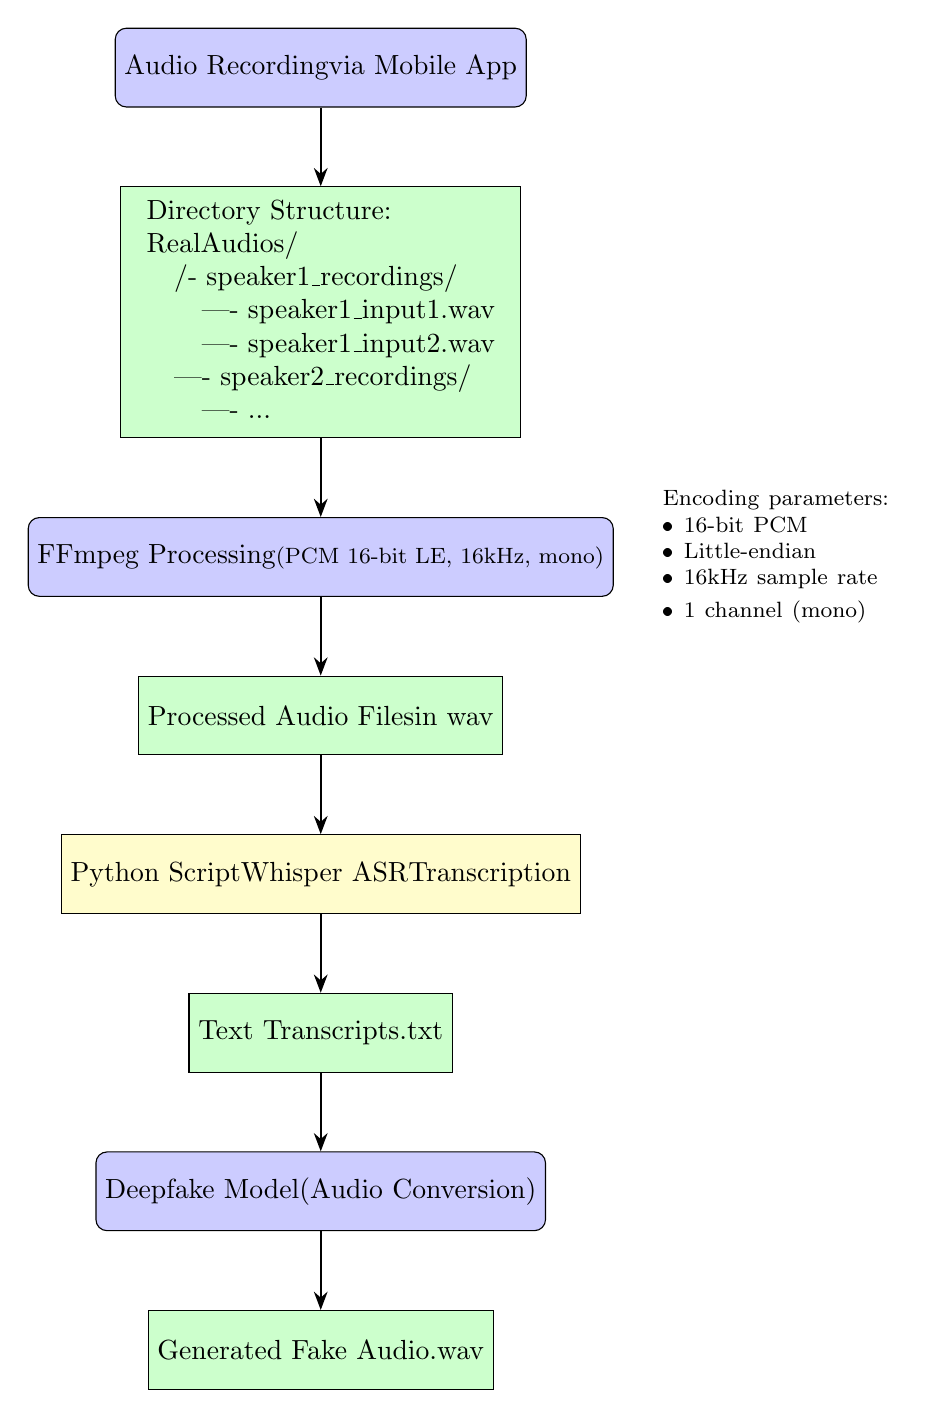
\begin{tikzpicture}[
    node distance=1cm,
    process/.style={rectangle, rounded corners, minimum width=3cm, minimum height=1cm, text centered, draw=black, fill=blue!20},
    data/.style={rectangle, minimum width=3cm, minimum height=1cm, text centered, draw=black, fill=green!20},
    script/.style={rectangle, minimum width=3cm, minimum height=1cm, text centered, draw=black, fill=yellow!20},
    arrow/.style={-Stealth, thick}
]

% Nodes
\node (record) [process] {Audio Recording\\via Mobile App};
\node (dirStruct) [data, below=of record] {
    \begin{tabular}{l}
        Directory Structure: \\
        RealAudios/ \\
        \quad /- speaker1\_recordings/ \\
        \quad \quad |- speaker1\_input1.wav \\
        \quad \quad |- speaker1\_input2.wav \\
        \quad |- speaker2\_recordings/ \\
        \quad \quad |- ...
    \end{tabular}
};

\node (ffmpeg) [process, below=of dirStruct] {FFmpeg Processing\\ 
    \footnotesize(PCM 16-bit LE, 16kHz, mono)};
    
\node (processedAudio) [data, below=of ffmpeg] {Processed Audio Files \\* in wav};

\node (whisper) [script, below=of processedAudio] {Python Script\\Whisper ASR\\Transcription};

\node (transcripts) [data, below=of whisper] {Text Transcripts\\*.txt};

\node (model) [process, below=of transcripts] {Deepfake Model\\(Audio Conversion)};

\node (fakeAudio) [data, below=of model] {Generated Fake Audio\\*.wav};

% Arrows
\draw [arrow] (record) -- (dirStruct);
\draw [arrow] (dirStruct) -- (ffmpeg);
\draw [arrow] (ffmpeg) -- (processedAudio);
\draw [arrow] (processedAudio) -- (whisper);
\draw [arrow] (whisper) -- (transcripts);
\draw [arrow] (transcripts) -- (model);
\draw [arrow] (model) -- (fakeAudio);

% Annotation
\node [right=0.5cm of ffmpeg, text width=3cm] {\footnotesize Encoding parameters: • 16-bit PCM\\• Little-endian\\• 16kHz sample rate\\• 1 channel (mono)};

\end{tikzpicture}
\end{document}
